% Adapted from the course-linked proposal template:
% https://www.overleaf.com/read/ddwygbxkfzkv
% Original aa228-jmlr2e.sty is included unchanged.
\documentclass[twoside,11pt]{article}
\usepackage{aa228-jmlr2e}
\usepackage{amsmath,booktabs}
\newcommand{\shorttitle}{Policy-Controlled Optimizers}
\begin{document}
\title{Policy-Controlled Optimizers under Biased Data Ordering}
% Individual contributions intentionally left blank for now.
% Nick Rui:
% Sandra Yang:
% Aidan Whitedeer:
\name{Nick Rui, Sandra Yang, and Aidan Whitedeer}
\renewcommand{\authorlist}{\normalsize\makebox[0pt][l]{\textbf{Nick Rui, Sandra Yang, and Aidan Whitedeer}}\\[3pt]
\small Status Update Draft --- November 13, 2026}
\renewcommand{\emaillist}{}
\maketitle

\paragraph{Problem and pivot.}
We are pivoting from segmentation correction to learned optimization: can a policy adapt hyperparameters to class-biased data ordering? Inspired by CS312, we study mixed data interrupted by biased blocks, then mixed data again.

\paragraph{Approach and progress.}
\textbf{Policy-Controlled Optimizers} learn hyperparameter policies in a partially observable Markov decision process. State contains weights, optimizer memory, and data-stream state. Policies observe time, controls, control-loss statistics, gradient norm, and gradient alignment with optimizer memory and the previous gradient. Actions are $(\eta,\mu,\lambda)$ for SGD, $(\eta,\beta_1,\beta_2,\lambda)$ for Adam/AdamW, and $(\eta,\mu,\alpha,\lambda)$ for RMSprop: learning rate, memory coefficients, and weight decay. Each action controls five updates; reward favors lower control loss. Future minibatches and block identities are unobserved.

Controllers have 16 hidden units and train with REINFORCE for 500 updates (4,000 episodes), with two policy seeds per optimizer. MNIST evaluation uses 200 gradient updates, ten orderings, and 20 paired episode seeds. Development data select checkpoints and constant-hyperparameter baselines; no test feedback.

\begin{center}
\small
\begin{tabular}{lrrrr}
\toprule
& \multicolumn{2}{c}{Random ordering} & \multicolumn{2}{c}{Biased orderings (mean)}\\
\cmidrule(lr){2-3}\cmidrule(lr){4-5}
Optimizer & Tuned fixed & Policy-controlled & Tuned fixed & Policy-controlled\\
\midrule
SGD & \textbf{92.27} & 92.25 & 88.36 & \textbf{89.13}\\
Adam & \textbf{92.63} & 92.52 & \textbf{91.50} & 90.69\\
AdamW & \textbf{92.63} & 92.40 & \textbf{91.50} & 90.51\\
RMSprop & 93.19 & \textbf{93.56} & 92.37 & \textbf{92.57}\\
\bottomrule
\end{tabular}\\[3pt]
Final test accuracy (\%); biased mean weights nine orderings equally.
\end{center}

\noindent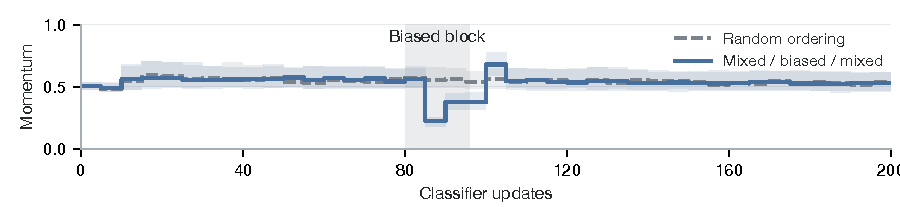
\includegraphics[width=\textwidth]{momentum_block.pdf}
{\small\noindent\textbf{Policy-Controlled SGD: learned momentum response.} Gray: single-digit block. Lines: medians; bands: middle 50\% of 20 episode seeds $\times$ two policy seeds (not confidence intervals).\par}

\paragraph{Findings and next steps.}
Momentum falls during bias and recovers afterward, showing reactivity, not its causal benefit. Biased-order gains are modest for SGD/RMSprop; Adam/AdamW decline. Two policy seeds, short episodes, and unequal total compute limit conclusions.

\paragraph{Timeline.}
\textbf{November:} ablations, simple controls, and additional seeds.
\textbf{By December 4:} consolidate findings and finish the report.
\end{document}
